\documentclass[12pt]{report}

\usepackage[utf8x]{inputenc}
\usepackage[T1]{fontenc}
\usepackage[frenchb]{babel}
\usepackage{lmodern}

\usepackage{amsmath,amsthm,amssymb}
\usepackage{graphicx}
\usepackage[colorinlistoftodos]{todonotes}
\usepackage{listings}
\usepackage{color}
\usepackage{verbatim}
\usepackage{grffile}


\definecolor{mygreen}{rgb}{0,0.6,0}
\definecolor{mygray}{rgb}{0.5,0.5,0.5}
\definecolor{mymauve}{rgb}{0.58,0,0.82}
\definecolor{darkWhite}{rgb}{0.94,0.94,0.94}

\lstset{
	aboveskip=3mm,
	belowskip=-2mm,
	backgroundcolor=\color{darkWhite},
	basicstyle=\footnotesize,
	breakatwhitespace=false,
	breaklines=true,
	captionpos=b,
	commentstyle=\color{red},
	deletekeywords={...},
	escapeinside={\%*}{*)},
	extendedchars=true,
	framexleftmargin=16pt,
	framextopmargin=3pt,
	framexbottommargin=6pt,
	frame=tb,
	keepspaces=true,
	keywordstyle=\color{blue},
	language=C,
	literate=
	{²}{{\textsuperscript{2}}}1
	{⁴}{{\textsuperscript{4}}}1
	{⁶}{{\textsuperscript{6}}}1
	{⁸}{{\textsuperscript{8}}}1
	{€}{{\euro{}}}1
	{é}{{\'e}}1
	{è}{{\`{e}}}1
	{ê}{{\^{e}}}1
	{ë}{{\¨{e}}}1
	{É}{{\'{E}}}1
	{Ê}{{\^{E}}}1
	{û}{{\^{u}}}1
	{ù}{{\`{u}}}1
	{â}{{\^{a}}}1
	{à}{{\`{a}}}1
	{á}{{\'{a}}}1
	{ã}{{\~{a}}}1
	{Á}{{\'{A}}}1
	{Â}{{\^{A}}}1
	{Ã}{{\~{A}}}1
	{ç}{{\c{c}}}1
	{Ç}{{\c{C}}}1
	{õ}{{\~{o}}}1
	{ó}{{\'{o}}}1
	{ô}{{\^{o}}}1
	{Õ}{{\~{O}}}1
	{Ó}{{\'{O}}}1
	{Ô}{{\^{O}}}1
	{î}{{\^{i}}}1
	{Î}{{\^{I}}}1
	{í}{{\'{i}}}1
	{Í}{{\~{Í}}}1,
	morekeywords={*,...},
	numbers=left,
	numbersep=10pt,
	numberstyle=\tiny\color{black},
	rulecolor=\color{black},
	showspaces=false,
	showstringspaces=false,
	showtabs=false,
	stepnumber=1,
	stringstyle=\color{gray},
	tabsize=4,
	title=\lstname,
}

\newtheorem{theo}{Théorème}[section]

\begin{document}

\begin{titlepage}

\newcommand{\HRule}{\rule{\linewidth}{0.5mm}} % Defines a new command for the horizontal lines, change thickness here

\begin{figure}
	\begin{minipage}[t]{.5\linewidth}
	\centering
	\includegraphics[scale=0.5]{esilv_logo.png}\\[1cm]
	\end{minipage}
	\begin{minipage}[t]{.5\linewidth}
	\includegraphics[scale=1.4]{edf_logo.png}\\[1cm]
	\end{minipage}
\end{figure}

\center % Center everything on the page


%	TITLE SECTION
%----------------------------------------------------------------------------------------

\HRule \\[0.4cm]
{ \huge \bfseries Pricer efficace d'actifs énergétiques}\\[0.4cm] % Title of your document
\HRule \\[1.5cm]

%----------------------------------------------------------------------------------------
%	AUTHOR SECTION
%----------------------------------------------------------------------------------------

\begin{minipage}{0.4\textwidth}
	\begin{flushleft} \large
		\emph{Team 16:}\\
		Anthony \textsc{Courillon} % Your name
		\\
		Denis \textsc{Barranco}
		\\
		Ousman \textsc{Asadullah}
		\\
		Hicham \textsc{Kortbi} % Your name
	\end{flushleft}
\end{minipage}
~
\begin{minipage}{0.4\textwidth}
	\begin{flushright} \large
		\emph{Partenaire:} \\
		Arnaud \textsc{de latour} % Supervisor's Name
		\\
		\emph{Mentor:} \\
		Martino \textsc{Grasselli} % Supervisor's Name
	\end{flushright}
\end{minipage}\\[2cm]

%----------------------------------------------------------------------------------------
%	DATE SECTION
%----------------------------------------------------------------------------------------

{\large Mars 2017}\\[2cm] % Date, change the \today to a set date if you want to be precise

\end{titlepage}


\chapter*{Introduction}
\addcontentsline{toc}{chapter}{Introduction}

Etant étudiants en quatrième année à l’ESILV dans la majeure finance et
dans le cadre du projet PI2, nous avons décidé de travailler sur la
réalisation d’un pricer d’actifs énergétiques proposé par notre partenaire EDF R\&D et encadré par Arnaud DE LATOUR

Un certain nombre d'actifs utilisés dans le domaine de l'énergie (par exemple les
centrales électriques) se prête facilement à une valorisation sous la forme de
produits dérivés complexes, de nature américaine (contrairement à une option
européenne, l'option américaine peut être exercée n'importe quand).

Le pricing de ces actifs met en oeuvre des méthodes numériques avancées qui
peuvent être coûteuses en temps de calcul. Lorsque ces méthodes sont fondées sur
une simulation Monte-Carlo (par exemple l'algorithme de Longstaff-Schwartz), on a
intérêt à employer des techniques de réduction de variance pour accélérer la
convergence de l'algorithme - et donc réduire le temps de calcul.

Cependant, l'efficacité de ces techniques dépend généralement du payoff de l'actif
qu'on cherche à valoriser. L'objectif de ce projet est donc d'implémenter et de
tester différentes méthodes de réduction de variance appliquées à des actifs
énergétiques, afin d'identifier les méthodes les plus pertinentes.

Nous allons réaliser ce pricer soous Python et nous allons utiliser exclusivement
ces 3 logiciels afin de réaliser ce projet:
\begin{itemize}
	\item Anaconda ;
	\item LiClipse ;
	\item Github.
\end{itemize}

\chapter{Evaluation du prix d'un produit dérivé par simulation}

\section{Principes des méthodes de Monte Carlo}

Le prix d'un produit dérivé d'un sous-jacent $X=(X_t)_{t\geq0}$ de payoff actualisé f(X), d'un marché financier sous probabilité risque neutre, s’écrit
comme l’espérance des flux futurs actualisés qu’il génère, $e_p$ :
\begin{equation}
	e_p = \mathbb{E}[f(X)]
\end{equation}
Il faut donc évaluer cette espérance pour connaître le prix d’un produit dérivé.
Nous allons utilize les méthodes de Monte Carlo qui consiste à simuler un grand
nombre de realisations, N indépendantes et identiquements distribuées, de f(X),
$f(X^i)$ avec $i\in \mathbb{N}$, puis on calcule chaque $f(X^i)$.

Enfin, on prend la moyenne empirique de ces réalisations, $\bar{e_N}$ estimateur de $e_p$ :
\begin{equation}
	\bar{e_N}=\frac{1}{N}\sum_{i=1}^{N} f(X^i) \xrightarrow[N\rightarrow{\infty}]{\text{p.s}} e_p \text{~avec~} \mathbb{E}[|f(X)|]<\infty
\end{equation}
la loi des grand nombres assure la convergence de $\bar{e_N}$ vers $e_p$.
Autrement dit, pour N assez grand, $\bar{e_N} \simeq e_p$.

\section{Limite pratique des méthodes de Monte Carlo}

\begin{theo}[Théorème Central Limite]\label{TCL}
	Nous allons utilisé le cas où on ne connait pas la loi de $e_p$.
	Si la loi de $e_p$ est inconnue (ou non normale), alors $\bar{e_N}\hookrightarrow N(\mu,\frac{\sigma}{\sqrt{N}})$ pour N assez grand, avec $\sigma$ = $\sqrt{(Var(f(X)))}$  et $\mu=e_p =\mathbb{E}[f(X)]$  alors on a:
	\begin{equation}
		\frac{\sqrt{N}(\bar{X}_n-\mu)}{\sigma}\hookrightarrow N(0,1)
	\end{equation}
\end{theo}

Donc le théorème central limite permet d'avoir l'approximation de l'erreur réalisée:
\begin{equation}
	\label{eq:approximation-erreur}
	\sqrt{N}(\frac{1}{N}\sum_{i=1}^{N}f(X^i)-e_p)\hookrightarrow N(0,\sqrt{Var(f(X))})
\end{equation}
ou :
\begin{equation}
	\sqrt{N}(\bar{e_N}-e_p)\hookrightarrow N(0,\sqrt{Var(f(X))})
\end{equation}

Cela montre le problème du nombre de simulations N nécessaires pour avoir un bon estimateur de $e_p$, plus la variance de $f(X^i)$ est élevé, plus N doit être grand.

Or N grand a pour conséquence une augmentation du temps de calcul. Donc plus $Var(f(X^i))$, plus l’obtention de l’évaluation de $e_p$ demandera un temps de calcul important.

Il est alors intéressant d’employer des techniques de réduction de variance pour accélérer la convergence de l’algorithme et donc réduire le temps de calcul. C’est l’un des problèmes que nous allons tenter de résoudre dans la réalisation de notre pricer.

Nous allons voir les différentes techniques de réduction de variance et tenter de les implémenter dans notre pricer dans le chapitre 2 de ce document.

\section{Contrôle de la convergence}

Il faut évaluer l’erreur d’approximation de \eqref{eq:approximation-erreur}  grâce à la construction d’un intervalle de confiance :
\begin{equation}
	Z = \frac{\sqrt{N}}{\sqrt{Var(f(X))}} (\frac{1}{N}\sum_{i=1}^{N}f(X^i)-e_p)\hookrightarrow N(0,1)
\end{equation}
En supposant que la variance est connue, on a :
\begin{equation}
	\mathbb{P}(-u\leq Z \leq u) = \alpha
\end{equation}
avec u fractile d'ordre 1-$\frac{\alpha}{2}$ de la N(0,1). Ce qui revient à :
\begin{equation}
	\mathbb{P}(-u \frac{\sqrt{Var(f(X))}}{\sqrt{N}}+\bar{e_N}\leq e_p \leq u \frac{\sqrt{Var(f(X))}}{\sqrt{N}}+\bar{e_N}) = \alpha
\end{equation}
et donc :
\begin{equation}
	\text{IC}_\alpha(e_p) = [-u \frac{\sqrt{Var(f(X))}}{\sqrt{N}}+\bar{e_N};u \frac{\sqrt{Var(f(X))}}{\sqrt{N}}+\bar{e_N}]
\end{equation}
L’erreur donné par un intervalle de confiance est :
\begin{equation}
	\mathbb{P}(e_p\in IC_\alpha ) \simeq \alpha
\end{equation}
Il a un problème c’est qu’on ne peut appliquer cette méthode que si la variance de f(X), Var(f(X)) est connue. Or ici, Var(f(X)) est inconnue, et il faut l’estimer grâce à un estimateur.

On peut construire un estimateur non biaisé tel que celui-ci :
\begin{equation}
	\bar{v_N} = \sqrt{\frac{1}{N-1}\sum_{i=1}^{N}(f(X^i)-\bar{e_N})^2}
\end{equation}

Voici l’implémentation sous Python de tout ce que nous avons énoncé dans cette partie I, dans le fichier $\_init\_.py$, on a pris  $\alpha$ =0.95 pour la contruction des intervalles de confiance.

\begin{lstlisting}
"Pricing d'actifs énergétiques par Monte Carlo."

import numpy as np
import pandas as pd
import scipy.stats as sps
import efficientmc.assets as assets
import efficientmc.pricemodels as pricemodels
import efficientmc.generators as generators
from collections import namedtuple

MCResults = namedtuple('MCResults', ('mean', 'iclow', 'icup'))

def runmc(*allassets):
"""
Calcule par simulation Monte-Carlo les cash-flows des actifs de
`allassets`, sous la probabilité risque-neutre.
"""
allmarkets = set([m for asset in allassets for m in asset.getmarkets()])
marketsdates = set([d for market in allmarkets for d in market.getdates()])
assetsdates = set([d for asset in allassets for d in asset.getdates()])
earnings = {asset.name: {} for asset in allassets}
prices = {market.name: {} for market in allmarkets}
volumes = {asset.name: {m.name: {} for m in asset.getmarkets()} \
for asset in allassets}
alldates = assetsdates.union(marketsdates)
for date in alldates:
#FIXME: utiliser une notion de `computation` pour sauvegarder et
# aggréger les résultats au fur et à mesure.
# Mise à jour des marchés :
for market in allmarkets:
market.simulate(date)
# Mise à jour des objets :
for asset in allassets:
earnings[asset.name][date] = asset.get_discounted_cf(date)
for market in asset.getmarkets():
volumes[asset.name][market.name][date] = asset.getvolume(date,
market)
#FIXME: on peut avoir besoin d'autre chose que du spot.
if date not in prices[market.name]:
prices[market.name][date] = market.getspot(date)
earnings = pd.Panel(earnings).transpose(1, 0, 2)
#FIXME: utiliser xarray.
volumes = {key: pd.Panel(value).transpose(1, 0, 2)
for key, value in volumes.items()}
prices = pd.Panel(prices).transpose(1, 0, 2)
return earnings, volumes, prices

def getmtm(cf, alpha=0.95):
"""
Calcule la MtM (i.e. : les cash-flows moyens réalisés et un intervalle
de confiance) de chaque actif listé dans `cf`.

Paramètres
----------
cf : pandas.Panel
Cash-flows réalisés pour chaque simulation (`items`), chaque
actif (`major_axis`) et chaque date (`minor_axis`).
alpha : double compris entre 0. et 1.
Quantile à utiliser pour le calcul des intervalles de confiances.
"""
nsims = cf.shape[0]
cumvalues = cf.sum(axis=2)
mean = cumvalues.mean(axis=1)
std = cumvalues.std(axis=1)
res = {}
for key, val in mean.items():
res[key] = mkmcresults(val, std[key], nsims)
return res

\end{lstlisting}

Il reste aussi le problème de la queue de distribution de
la veritable loi de $\bar{e_N}$  (on a supposé précedemment qu'elle suivait une loi normale grâce au TCL) qui n’est pas négligeable, nous verrons cela plus en détails à travers les résultats obtenus de notre pricer.\\\\
Il y a par exemple, le prix de l’électricité en forward
qui varie extrêmement et ne fluctue plus comme une loi
gaussienne. La distribution de ses fluctuations
appartient au régime des distributions dites « à queue
épaisse ».\\\\
Nous verrons cela dans le chapitre 3 et 4 de ce rapport.
\newpage
\section{Générateur aléatoire}
On a besoin de simuler des variables aléatoires. Or un
ordinateur ne génère que de suites déterministes.
bruit gaussien: realisation de processus aléatoire suivant une loi normale)
Sous Python, nous allons stocké des bruits gaussiens dans un tableau (matrice).
Voici la classe GaussianGenerator dans le fichier generators.py correspondant :

\begin{lstlisting}
	import numpy as np
	from efficientmc.utils import timecached, DateCache
	import sobol_seq
	import ghalton as gh
	from scipy.stats import norm
	from math import ceil, fmod, floor, log
	
	class GaussianGenerator:
	"Générateur de bruits gaussiens corrélés."
	
	def __init__(self, nsims, corrmatrix, corrkeys, randomfunc):
	"""
	Initialise une nouvelle instance de la classe `GaussianGenerator`.
	
	Paramètres :
	------------
	nsims : entier positif
	Nombre de simulations à générer.
	corrmatrix : matrice carrée
	Matrice de corrélation entre les différents bruits gaussiens
	à simuler. La matrice doit être définie positive.
	corrkeys
	Liste des identifiants associés aux différentes lignes / colonnes
	de la matrice de corrélation `corrmatrix`. Les identifiants doivent
	être donnés dans l'ordre dans lequel les bruits correspondants
	apparaissent dans `corrmatrix`.
	randomfunc
	Fonction permettant de générer des bruits gaussiens indépendants
	(typiquement `np.random.randn`).
	"""
	self.corrmatrix = corrmatrix
	self.corrkeys = corrkeys
	self.nsims = nsims
	self.randomfunc = randomfunc
	self.cache = DateCache()
	try:
	np.linalg.cholesky(self.corrmatrix)
	except np.linalg.LinAlgError:
	raise np.linalg.LinAlgError("the correlation matrix is not "\
	"positive definite.") from None
	
	@property
	def nnoises(self):
	"Nombre de bruits gaussiens distincts à simuler."
	return self.corrmatrix.shape[0]
	
	@timecached
	def getallnoises(self, date):
	"""
	Renvoie `self.nsims` réalisations de `self.nnoises` bruits
	gaussiens corrélés.
	"""
	whitenoises = self.randomfunc(self.nnoises, self.nsims)
	noises = np.dot(np.linalg.cholesky(self.corrmatrix), whitenoises)
	return noises
	
	@timecached
	def getnoises(self, date, keys):
	"""
	Renvoie un tableau de taille `(len(keys), self.nsims)` de bruits
	gaussiens corrélés correspondants aux aléas identifiés par les
	clefs `keys`.
	"""
	noises = self.getallnoises(date)
	res = np.empty((len(keys), self.nsims))
	for idx, key in enumerate(keys):
	keyidx = self.corrkeys.index(key)
	res[idx, :] = noises[keyidx, :]
	return res
	
\end{lstlisting}

\chapter{Méthodes de réduction de la variance}
\section{Variables antitthétiques}
L’idée des variables antithétiques repose sur la symétrie de la
distribution de la loi uniforme et la correlation entre 2
variables aléatoires.
\subsection{Idées globales}
Calculer $\theta$ = $\text{E}[Y]$=$\text{E}[f(X)]$\\
$\text{E}[Y]$=$\frac{1}{2}$$\text{E}[Y_1]+\text{E}[Y_2]=\text{E}[\frac{Y_1+Y_2}{2}]$\\
Var($\frac{Y_1+Y_2}{2})=\frac{Var(Y_1)+Var(Y_2)+2Cov(Y_1,Y_2)}{4}$\\
- Si $Y_1$ et $Y_2$ sont indépendantes, Cov($Y_1,Y_2$)=0\\
-Si Cov($Y_1,Y_2$)<0, alors $Var(\frac{Y_1+Y_2}{2})<Var(\frac{Y}{2})$ donc la variante est réduite si $Y_1$ et $Y_2$ sont corrélés négativements, Cov($Y_1,Y_2)<$0\\\\
\subsection{Mathématiquement}
On veut estimer $\text{E}[Y]$ en utilisant l'implémentation d'échantillons antithétiques c'est-à-dire: $(Y_1,Y_{1ant}),(Y_2,Y_{2ant}),...,(Y_N,Y_{Nant})$  avec $\forall$ i $\in$ $\mathbb{N}$, $Y_i$ et $Y_{iant}$ de même loi de distribution et i.i.d. (indépendantes et identiquement distribuées).\\
L'estimateur de $\text{E}[Y]$ est simplement la moyene des 2N réalisations:\\\\
$\bar{e_{Nant}}$=$\frac{1}{2N}(\sum_{i=1}^{N}Y_i +\sum_{i=1}^{N}Y_{iant})$=$\frac{1}{N}\sum_{i=1}^{N}(\frac{Y_i+Y_{iant}}{2})$\\\\
En utilisant les mêmes méthodes que dans le chapitre I, on par TCL:\\
\begin{center}
	$\frac{\sqrt{N}(\bar{e}_{Nant}-\text{E}[Y])}{\sqrt{Var(Y)}}$
\end{center}
On pose $\sigma^2_{ant}=Var(Y)=Var(\frac{Y_i+Y_{iant}}{2})$\\\\
Comme nous venons de le voir dans les idées globales:\\\\
$\sigma^2_{ant}=\frac{Var(Y_i)+Var(Y_{iant})+2Cov(Y_i,Y_{iant})}{4}$\\\\
$ =\frac{2Var(Y_i)+2Cov(Y_i,Y_{iant})}{4}$ car $Y_i $ et $ Y_{iant}$ sont de même loi de distribution\\\\
$=\frac{Var(Y_i)+2Cov(Y_i,Y_{iant})}{2}$\\\\
Alors, si $Cov(Y_i,Y_{iant}) <0$, $\sigma^2<\frac{Var(Y_i)}{2}$\\\\
Donc nous avons besoin de construire les paires $Y_i$ et $Y_{iant}$ de façon à ce que $Cov(Y_i,Y_{iant}) <0$ pour réduire la variance.\\\\
\subsection{Implémentation}
Comme nous simulons une matrice de bruits gaussiens indépendants, on peut implémenter la méthode des variables antithétiques en construisant une séquence $Y_i,Y_2,...,Y_N$ (rappel: $f(X^i)$ avec i $\in \mathbb{N})$ puis construire une autre séquence opposé à la première en prenant la négation de celle-ci: $-Y_1,-Y_2,...,-Y_N.$\\\\
Pseudo-code:\\
1. Créer une matrice vide de taille (nnoises,nsims) avec \\nnoises: nombre de bruits gaussiens indépendants \\ nsims: nombre de simulations\\
2. Générer dans la moitié de la matrice des bruits gaussiens.\\
3. Prendre l'opposé de la première moitié de la matrice, pour remplir la deuxième moitié de la matrice.\\\\
Voici l'implémentation sous Python de la méthode des variables antithétiques:
\begin{lstlisting}
def antithetic_randn(nnoises, nsims):
"""
Renvoie un tableau de bruits gaussiens non corrélés :math:`(G_{_i,j})`
de taille `(nnoises, nsims)`, et tel que, pour tout :math:`i` :
:math:`\forall 1 \leq j \leq n / 2, G_{i,n/2+j} = -G_{i,j}`

Paramètres :
------------
nnoises : entier positif
Nombre de bruits à simuler.
nsims : entier positif, pair
Nombre de simulations à effectuer par prix.
"""
if nsims % 2 != 0:
raise ValueError("the number of simulations used with antithetic "\
"variables should be even.")
half = int(0.5 * nsims)
noises = np.empty((nnoises,nsims))
noises[:, :half] = np.random.randn(nnoises, half)
noises[:, half:] = -noises[:, :half]
return noises

\end{lstlisting}
\newpage
\section{Suites à discrépance faible (Quasi Monte Carlo)}
Nous allons étudier les méthodes de Quasi Monte Carlo qui contrairement au Monte Carlo classique n'est pas basé sur la génération de nombres pseudo-aléatoires mais sur la génération de nombre déterministe aux propriétés spéciales générés par des suites à discrépance faible.//
On peut voir le problème de l'évaluation du prix d'un produit dérivé vu dans le chapitre I (1)  comme une intégrale à la place d'une espérance:\\\\
$e_p^{QMC}=$$\int_{[0,1]^s} f(u) \, \mathrm du$=$\frac{1}{N}\sum_{i=1}^{N}f(X^i)$\\\\
On cherche à approximer l'intégrale.\\
Pour cela, il faut générer les points $X^i$ dans l'hypercube $[0,1]^s$ avec s la dimension de l'espace.
Ces points doivent être équiréparties.
On ne se souciait pas vraiment de la dimension jusqu'à présent mais plus la dimension sera grande, plus il y aura des irrégularités dans les projections.\\
Nous allons voir les différentes suites à discrépance faible permettant de générer ces points.


Discrépance et propriétés d'équirépartition à détailler.(a faire)
\subsection{Suite de Van Der Corput}

La suite de Van der Corput génère une suite de points dans l'intervalle [0,1] qui ne se répète jamais.\\
La suite de Van der Corput en base b est de la forme:\\
$\phi_b(n)=\frac{a_o}{b}+\frac{a_1}{b^2}+...+\frac{a_r}{b^{r+1}}$\\ avec n=$a_0+a_1+...+a_rb^r$, $a_r>0$, $0\leq a_i \leq p$, $0\leq i \leq r$
\begin{center}
	ou \\
\end{center}
$\phi_b: \mathbb{N} \rightarrow[0,1)$]\\
$\forall$ $ b\in \mathbb{N}$, $\phi_b(n)=\sum_{i=0}^{I}\frac{a_i(n,b)}{b^{i-1}}$\\\\

Nous allons voir les suites de Van Der Corput avec deux exemples ayant chacun leur approche. C'est important de bien comprendre cette suite car elle est la clé de la compréhension des suites qui vont suivre.\\\\

\subsubsection{Exemple 1: l'approche classique}
Nous allons prendre un exemple d'une suite de Van Der Corput en base 2 distribué sur l'intervalle [0,1).\\
Pour n=12, les nombres générés sont: 0,$\frac{1}{2},\frac{1}{4},\frac{3}{4},\frac{1}{8},\frac{5}{8},\frac{3}{8},\frac{7}{8},\frac{1}{16},\frac{9}{16},\frac{5}{16},\frac{13}{16}$\\
\bigbreak
\begin{figure}[h]
	\begin{center}
	\includegraphics[scale=0.5]{figure1-van-der-corput.png}\\
	\end{center}
\caption{Suite de Van Der Corput en base 2 pour n=12}
\end{figure}
Les nombres générés séquentiellement remplissent les larges espaces entre les nombres précédents de la séquence.\\
\\En prenant la logique de la construction d'une suite de Van Der Corput, nous avons implémenté sous Python les fonctions permmettant de générer la séquence:\\
\begin{lstlisting}
def vdc(n, base):
"""
Cette fonction permet de calculer le n-ieme nombre de la base b de la 
séquence de Van Der Corput
"""
vdc, denom = 0,1
while n:
denom *= base
n, remainder = divmod(n, base)
vdc += remainder / denom
return vdc
\end{lstlisting}
\bigbreak

\begin{lstlisting}
def van_der_corput(nsims,b):
"""
Cette fonction permet de générer la séquence de Van Der Corput en base b
"""
array=np.empty(nsims)
i=0
for i in range(nsims):
array[i]=vdc(i,b)
return array
\end{lstlisting}
On a testé ces fonctions et on a tracé ceci:\\
\begin{figure}[h]
	\begin{center}
		\includegraphics[scale=0.5]{figure_1-van_der_corput_exemple1.png}\\
	\end{center}
	\caption{Suite de Van Der Corput en base 2 pour n=30}
\end{figure}
\medbreak
On voit bien sur la figure 2.2 que le points générés par la séquence de Van Der Corput sont plutôt bien équiréparties.
\subsubsection{Exemple 2:l'approche binaire}
On peut calculer le n-ième terme de la suite de Van Der Corput de base b comme ceci:
\begin{figure}[h]
	\begin{center}
		\includegraphics[scale=0.5]{figure2.3-van_der_corput_binaire.png}\\
	\end{center}
	\caption{Suite de Van Der Corput en base 2 pour n=30}
\end{figure}
$\phi_b(n)=\sum_{i=0}^{I}\frac{a_i(n)}{b^{i-1}}$\\\\
Les $a_i(n)$ sont la réflexion de n en une base b.\\
I=int(ln(n)/ln(b).\\
ex:\\
n=19 et b=3, $19=2\times3^2+0\times3^1+1\times3^0$\\
$\phi_3(19)=\frac{1}{3}+\frac{0}{9}+\frac{2}{27}=\frac{11}{27}$
\subsubsection{Implémentation de la suite de Van Der Corput}
Voici l'implémentation sous Python.\\
\begin{lstlisting}
	def vdc(n, base):
	"""
	Cette fonction permet de calculer le n-ieme nombre de la base b de la 
	séquence de Van Der Corput
	"""
	vdc, denom = 0,1
	while n:
	denom *= base
	n, remainder = divmod(n, base)
	vdc += remainder / denom
	return norm.ppf(vdc)
	
	def van_der_corput(nsims,b):
	"""
	Cette fonction permet de générer la séquence de Van Der Corput en base b
	"""
	array=np.empty(nsims)
	i=0
	for i in range(nsims):
	array[i]=vdc(i,b)
	return array
	
	def van_der_corput_dimension(dim,nsims):
	array=np.empty((dim,nsims))
	"""
	Cette fonction génère dans un tableau de taille (dim,nsims) toutes les séquences
	de la suite de Van der Corput de la base 2 à la base dim+2
	"""
	for i in range(2,dim+2,1):
	array[i-2,:]=van_der_corput(nsims, i)
	return array
	
\end{lstlisting}
\subsubsection{Discrépance}
$D_N^*(\phi_b(1),\phi_b(2),...,\phi_b(N))= \mathcal{O}(\frac{logN}{N})$ \\
avec N=nsims nombres de simulations.
\newpage

\subsection{Suite de Halton}

La suite de Halton est une extension de la suite de Van der Corput en plusieurs dimensions.\\
Elle est composée de d 1-dimension suites de Van der Corput en utilisant comme base les premiers nombres premiers.\\
Un point généré par la suite de Halton est de la forme:\\
$x_i=(\phi_{p_1}(i),\phi_{p_2}(i),...,\phi{p_d}(i))$\\
avec d la dimension de la suite de Halton et $p_1,p_2,...,p_d$ les premiers nombres premiers.\\

\subsubsection{Implémentation de la suite de Halton}
En prenant la logique de la construction de la suite de Halton, nous l'avons implémenté de 2 façons, dont voici la première :\\
\begin{lstlisting}
def haltonF(nnoises,nsims):
Prime=[2, 3, 5, 7, 11, 13, 17, 19, 23, 29, 31, 37, 41, 43, 47, 53,\
59, 61, 67, 71, 73, 79, 83, 89, 97, 101, 103, 107, 109, 113,\
127, 131, 137, 139, 149, 151, 157, 163, 167, 173, 179, 181,\
191, 193, 197, 199, 211, 223, 227, 229, 233, 239, 241, 251,\
257, 263, 269, 271, 277, 281]
halton=np.empty((nnoises,nsims))
for i in range(0,nsims,1):
for j in range(0,nnoises,1):
prime=Prime[j]
halton[j,i]=vdc(i,prime)
return halton
\end{lstlisting}
Elle suit la logique décrite précedemment.\\
\newpage
Sous Python, la suite de Halton est déjà existante dans le module ghalton. Voici la deuxième implémentation:\\
\begin{lstlisting}
import ghalton as gh
def halton(dim,nsims):
"""
Attention: la fonction crash pour nsims>500, on doit revoir l'optimisation de la fonction

On utilise la librairie Python existante sur la suite de Halton

GeneralizedHalton produit une suite de nsims dimension (colonnes),
le nombre 68 est utilisé pour faire des permutations, c'est le nombre qui permet de se rapprocher
le plus des valeurs du Monte Carlo classique
"""
sequence = gh.GeneralizedHalton(nsims,68)
"Une liste de dim sous-listes est produite"
points=sequence.get(dim)
"Pour lire la liste dans une matrice à plusieurs dimensions (dim,nsims)"
data=np.array(norm.ppf(points))
shape=(dim,nsims)
return data.reshape(shape)
\end{lstlisting}
La suite que nous avons construite marche beaucoup mieux que celle existante. (problème d'allocation de la mémoire, ghalton pas assez optimisé).
\newpage
Il est intéressant de comparer la suite de Halton avec une génération aléatoire simple. (Monte Carlo classique)\\

On génère le même nombre de points dans les 2 cas.\\
\begin{figure}[!h]
\centering
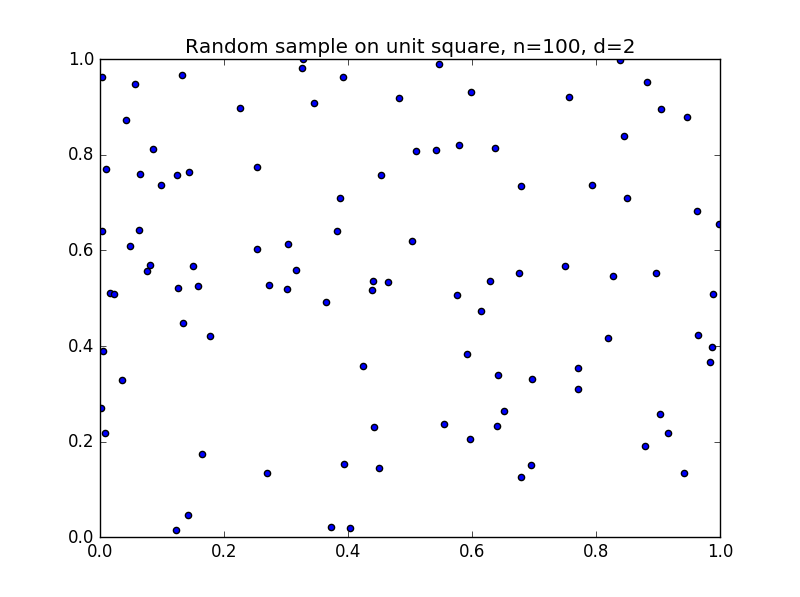
\includegraphics[scale=0.5]{figure_2-halton-random-sample.png}
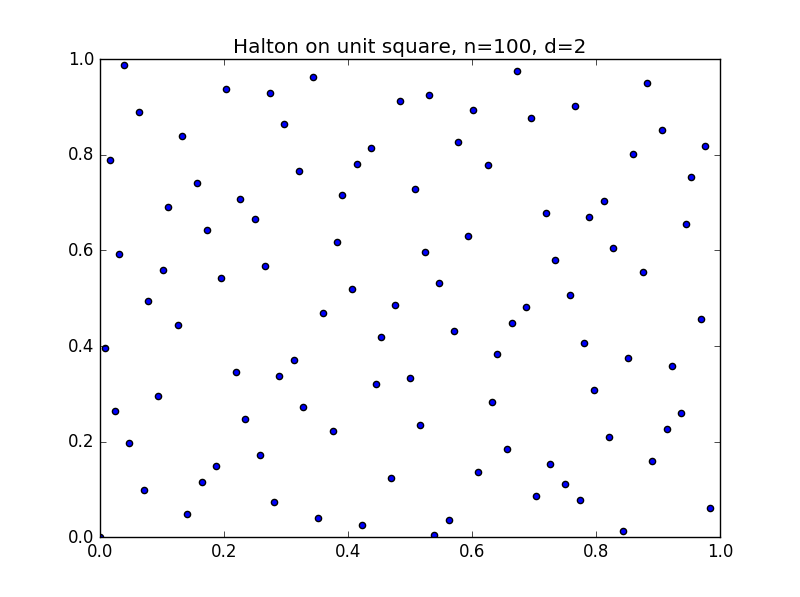
\includegraphics[scale=0.5]{figure_2-halton-halton.png}
\caption{Comparaison Monte Carlo classique et suite de Halton}
\end{figure}

On voit bien la différence et les propriétés d'équirépartition des points générés par la suite de Halton.
Malheureusement, plus la dimension devient grande, plus la suite de Halton de Halton marche moins.\\\\
La génération de points équiréparties dans l'intervalle $[0,1)^d$ devient plus difficile quand d la dimension augmente car l'espace à remplir devient trop large.\\\\
Dans notre cas, la suite de Halton marche plutôt bien jusqu'à d=8.\\

\begin{figure}[!h]
\centering
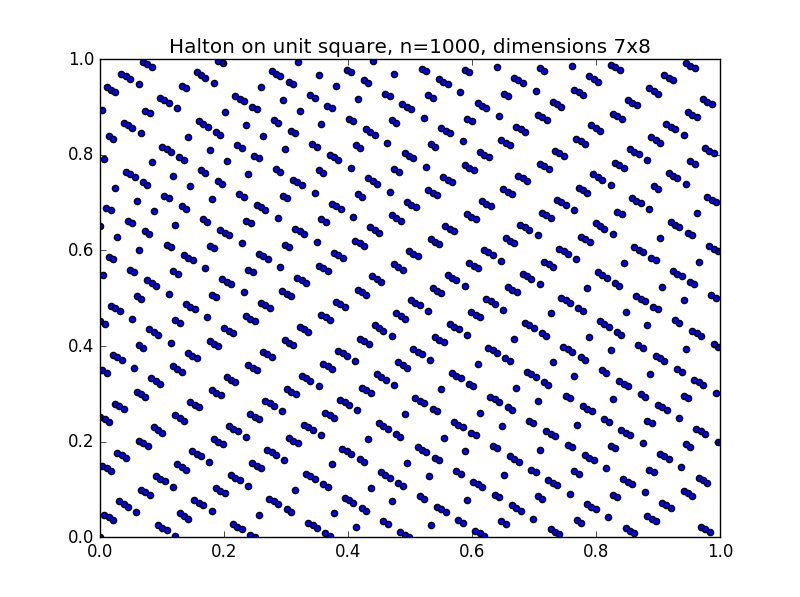
\includegraphics[scale=0.5]{figure_2-halton-dimensions 6 8.png}
\end{figure}
\newpage
Après la dimension d=14, la suite de Halton laisse des grands espaces.
\begin{figure}[!h]
\centering
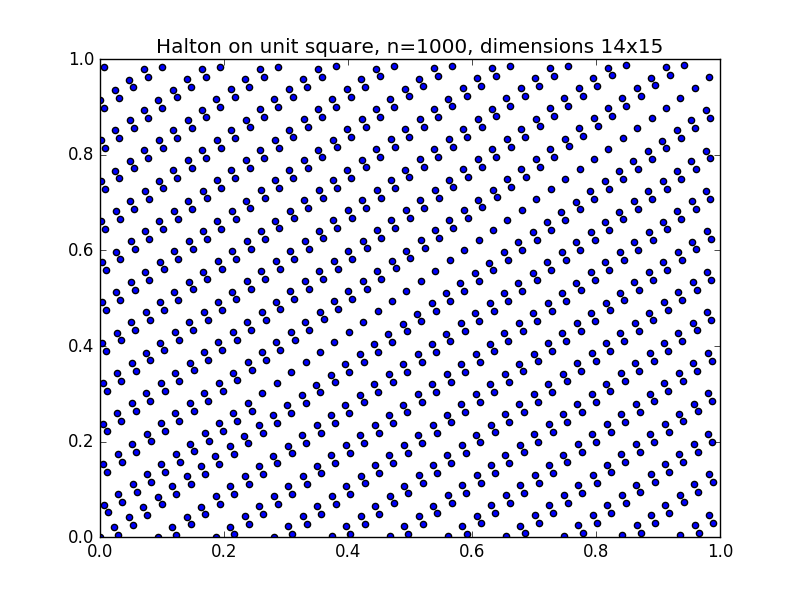
\includegraphics[scale=0.5]{figure_2-halton-dimensions 14 15.png}
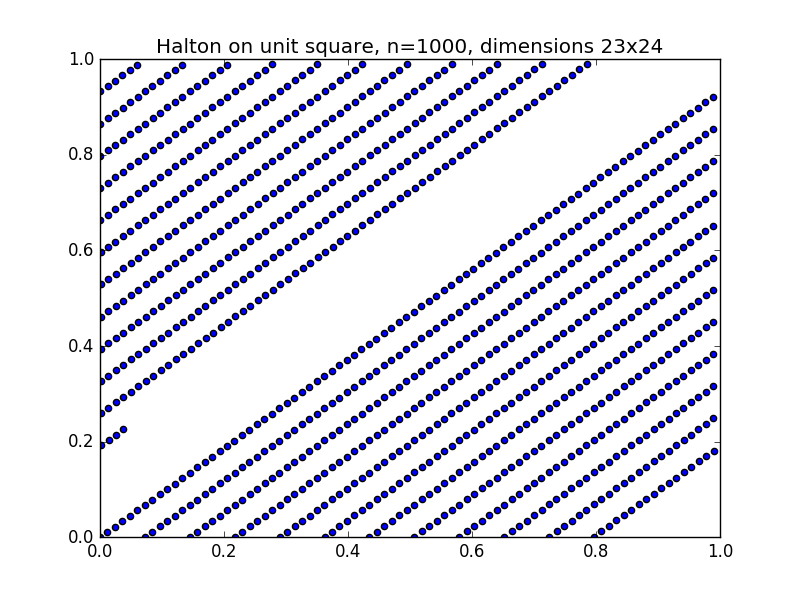
\includegraphics[scale=0.5]{figure_2-halton-dimensions 23 24.png}	
\caption{Faiblesse de la suite de Halton en grandes dimensions}
\end{figure}

\subsubsection{Discrépance}
$D_N^*(x_1,x_2,...,x_N)=\mathcal{O}(\frac{(logN)^d}{N}) $\\
d la dimension de la suite de halton tel que: $p_1,p_2,...,p_d$ d premiers nombres premiers et N=nsims nombre de simulations.
\newpage

\subsection{Suite de Hammersley}
La suite de Hammersely est une simple modification de la suite de Halton. Elle est de la forme:\\
$x_i=(i/n,\phi_{p1}(i),\phi_{p2}(i),...,\phi_{d-1}(i))$


\subsubsection{Discrépance}
L'avantage par rapport à la suite de Halton est que la discrépance est meilleure pour Hammersley.
$D_N^*(x_1,x_2,...,x_N)=\mathcal{O}(\frac{(logN)^d-1}{N} $\\
d la dimension de la suite de halton tel que: $p_1,p_2,...,p_{d-1}$ d-1 premiers nombres premiers et N=nsims nombre de simulations.

\subsubsection{Implémentation de la suite de Hammersley}
\begin{lstlisting}
	def hammersley(nnoises,nsims):
	Prime=[2, 3, 5, 7, 11, 13, 17, 19, 23, 29, 31, 37, 41, 43, 47, 53,\
	59, 61, 67, 71, 73, 79, 83, 89, 97, 101, 103, 107, 109, 113,\
	127, 131, 137, 139, 149, 151, 157, 163, 167, 173, 179, 181,\
	191, 193, 197, 199, 211, 223, 227, 229, 233, 239, 241, 251,\
	257, 263, 269, 271, 277, 281]
	hammersley=np.empty((nnoises,nsims))
	for i in range(0,nsims,1):
	hammersley[0,i]=i/nsims
	for i in range(0,nsims,1):
	for j in range(1,nnoises-1,1):
	prime=Prime[j]
	hammersley[j,i]=vdc(i,prime)
	return hammersley
\end{lstlisting}
\newpage
\subsubsection{Remarque}
La suite de Hammersley ne sera utile que en moyenne dimensions et ne sera donc pas intrès intéressante pour nous à cause de la séquence de la 1ère dimension.\\
Nous l'avons quand même implémenté vu la simple modification de la suite de Halton pour avoir une comparaison entre plusieurs suites à discrépances faibles.

Voici la comparaison entre une génération aléatoire simple, la suite de Halton et la suite de Hammersley:\\\\

\begin{figure}[h]
	\centering
	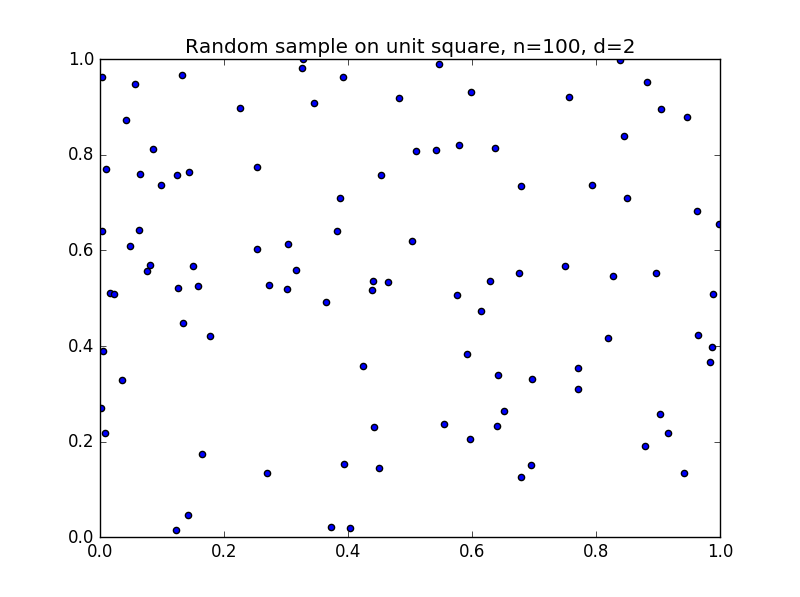
\includegraphics[scale=0.4]{figure_2-halton-random-sample.png}
	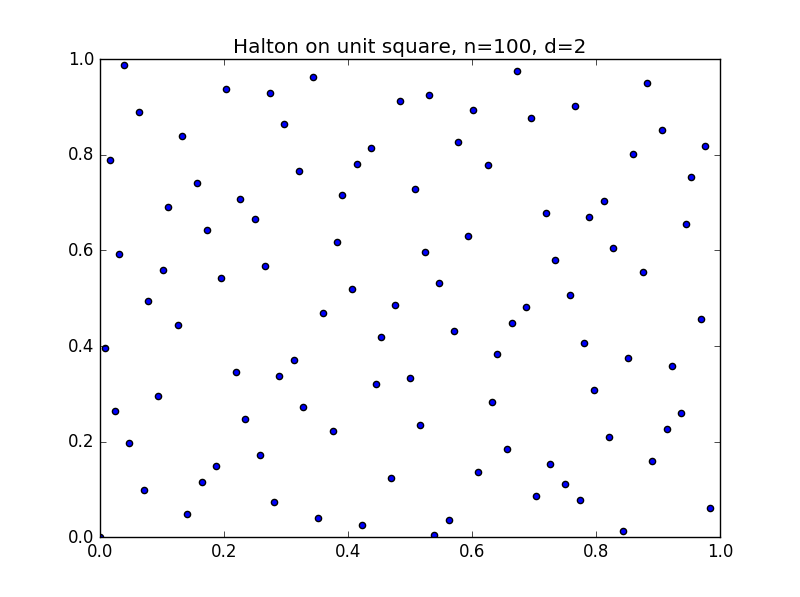
\includegraphics[scale=0.4]{figure_2-halton-halton.png}
	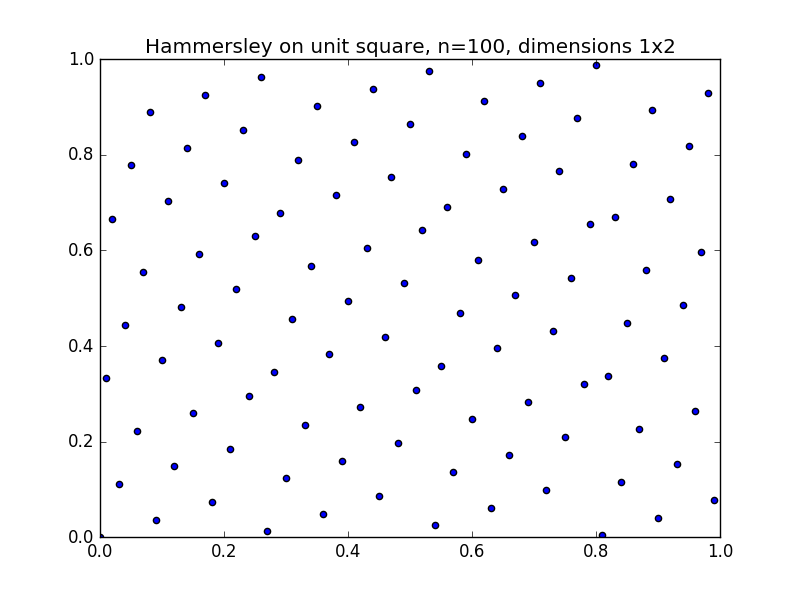
\includegraphics[scale=0.4]{figure_3-hammersley.png}
	\caption{Comparaisons Monte Carlo classique-Suite de Halton-Suite de Hammersley}	
\end{figure}

\clearpage
\subsection{Suite de faure}
  La suite de Faure  d-dimension utilise le plus petit nombre premier tel que p$\geq d$ avec p nombre premier.\\
La suite de Faure à d-dimensions est donné par la formule suivante:\\
$x_n=(\phi_r(n),T(\phi_r(n),...,T^{d-1}(\phi_r(n)))$\\
avec $\phi_r$ la suite de Van der Corput en base r et T la transformation dépendant des coefficients binomiaux et la décomposition de n en base r.\\
Pour la suite de Van der Corput:\\
$\phi_r^1(n)=\sum{i=0}{I}\frac{a_i^1(n)}{r^{i+1}}.$ avec I= partie entière de (ln(n)/ln(r))\\
La transformation de la suite de Van der Corput en base r se fait de la manière suivante:\\
$a_i^d(n)=\sum{j=1}{I}{i \choose j}a_i^{d-1}(n) mod r$\\

D'après nos recherches, la suite de Faure permet contrairement à la suite de Halton en hautes dimensions de mieux remplir l'hypercube gràce a l'utilisation du plus petit nombre premier.\\
ex:\\
Halton d=55, la dernière suite de Halton utilise le 55ème nombre premier: 257\\
Faure d=55, le nombre premier utilisé est 59>257.\\\\
Malheuresement, la suite de Faure est très couteuse en temps.\\
Nous avons essayé d'implémenter cette suite pour voir les résultats mais à cause de la récursivité mal optimisé, la génération de la suite de Faure met trop de temps à ce générer au delà de la dimension 4.\\

\newpage
\subsubsection{Implémentation de la suite de Faure}
Voici l'implémentation de la suite de Faure:\\

\begin{lstlisting}
def toDigits2(n, b):
"""Convert a positive number n to its digit representation in base b."""
digits = []
while n > 0:
digits.insert(0, n % b)
n  = n // b
digits.reverse()
i=0
for i in range(0,len(digits),1):
digits[i]/=b**(i+1)
return digits

def toDigits3(n, b,dim):
if n!=0:
I=int(math.log(n)/math.log(b))+1
else:
I=0
z=[]
a=toDigits2(n,b)
if dim==1:
return a
else:
for i in range(0,I-1,1):
h=0
for j in range(i,I-1,1):
h+=(comb(i,j)*toDigits3(n,b,dim-1)[i])%b
z.append(h)
return z 

def sumDigits(n,b):
a=toDigits2(n,b)
return np.sum(a)

def faureF(dim,nsims):
array=np.empty((dim,nsims))
p=2
Prime=[2, 3, 5, 7, 11, 13, 17, 19, 23, 29, 31, 37, 41, 43, 47, 53,\
59, 61, 67, 71, 73, 79, 83, 89, 97, 101, 103, 107, 109, 113,\
127, 131, 137, 139, 149, 151, 157, 163, 167, 173, 179, 181,\
191, 193, 197, 199, 211, 223, 227, 229, 233, 239, 241, 251,\
257, 263, 269, 271, 277, 281]
i=0
for i in range(0,nsims,1):
array[0,i]=sumDigits(i,2)
if dim==1:
"Si la dimension est égale à 1, on prend 2 comme base"
return array
else:
i=0
while p<dim:
p=Prime[i+1]
j=0
s=1
for s in range(1,dim,1):
for j in range(0,nsims,1):
array[s,j]=np.sum(toDigits3(j,p,s+1))
return norm.ppf(array)
 
\end{lstlisting}

A refaire si il reste du temps.
\newpage

\subsection{Suite de Sobol}
    La suite de Sobol d-dimensions comme la suite de Faure a la même base pour toutes ces d-dimensions, utilisant la base 2 et elle permute les élements dans chaque dimension grâce à une série de "nombres dirigés" $V_i$.\\\\
$V_i=\frac{m_i}{2^i}$ où les $ m_i$ sont des entiers paires positifs inférieures à $2^i$.\\\\
La suite de Sobol d-dimension est de la forme suivante:\\\\
$x_n=(a_1(n)V_1\textcircled{+},...,\textcircled{+}a_r(n))$

\subsubsection{Implémentation}
\begin{lstlisting}
	def sobolF(nnoises,nsims):
	"""
	Renvoie un tableau de valeurs générés par la suite de Sobol
	de taille (nnoises,nsims)
	"""
	noises = np.empty((nnoises,nsims))
	#  Utilisation de la fonction sobol_seq.i4_sobol_generate_std_normal
	# pour générer des variables quasi-aléatoires suivant une loi normale.
	noises = sobol_seq.i4_sobol_generate_std_normal(nnoises, nsims)
	noises=np.transpose(noises)
	return noises
\end{lstlisting}
\newpage


\begin{figure}[h]
	\centering
	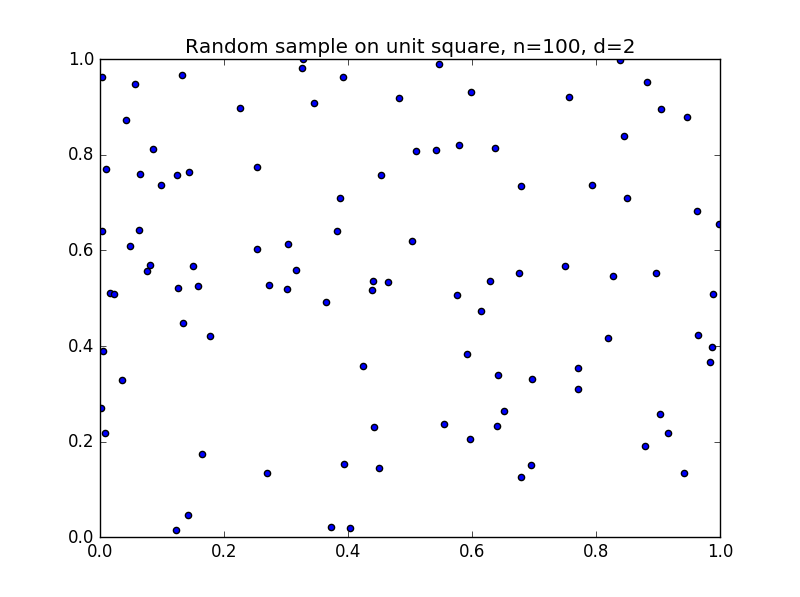
\includegraphics[scale=0.5]{figure_2-halton-random-sample.png}
	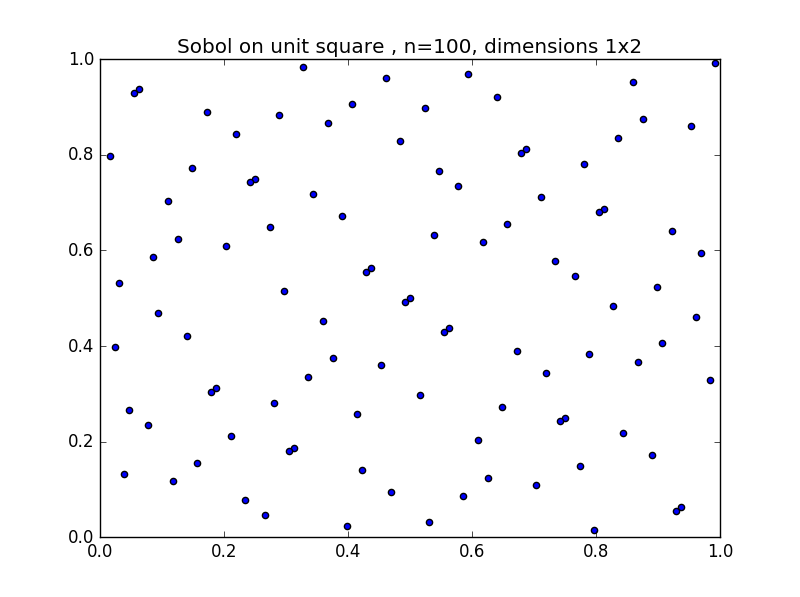
\includegraphics[scale=0.5]{figure_4-sobol.png}
	\caption{Comparaisons Monte Carlo classique - Suite de Sobol}	
\end{figure}

\clearpage

\begin{figure}[h]
	\centering
	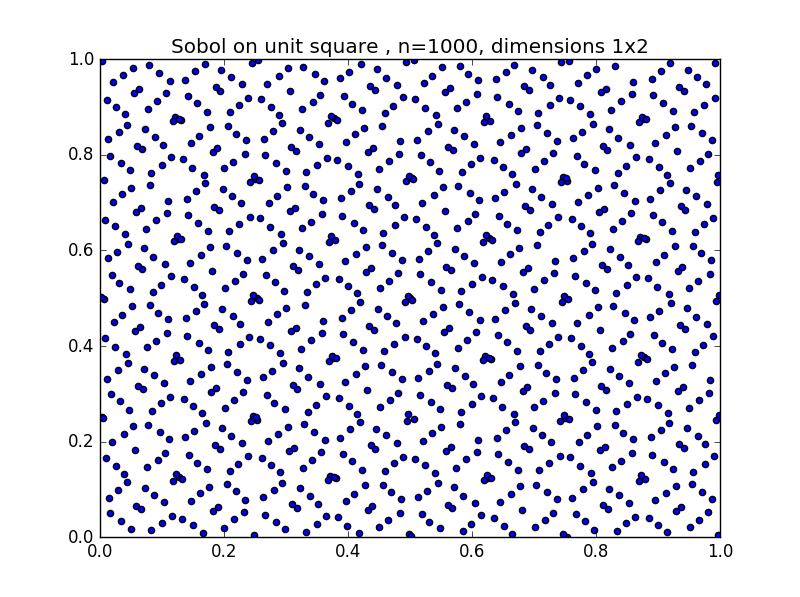
\includegraphics[scale=0.4]{figure_4-sobol 1000 dimensions 1x2.png}
	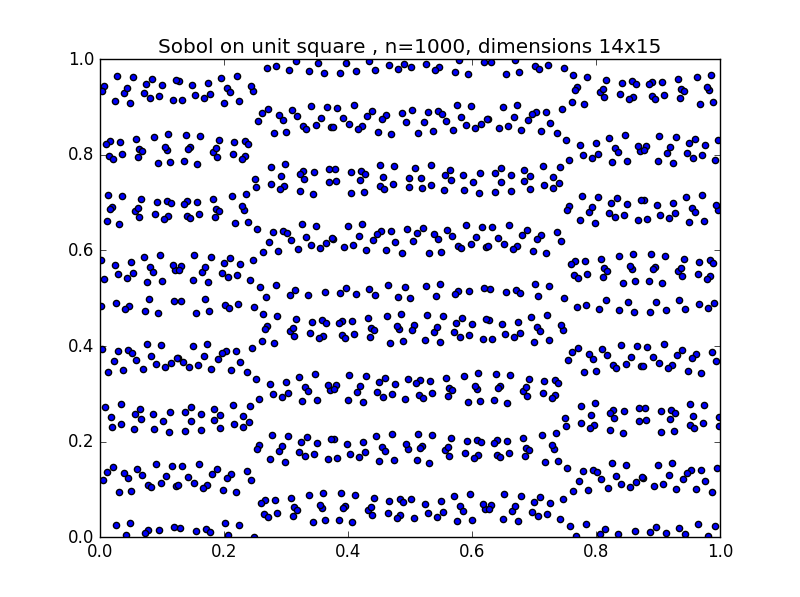
\includegraphics[scale=0.4]{figure_4-sobol 1000 dimensions 14x15.png}
	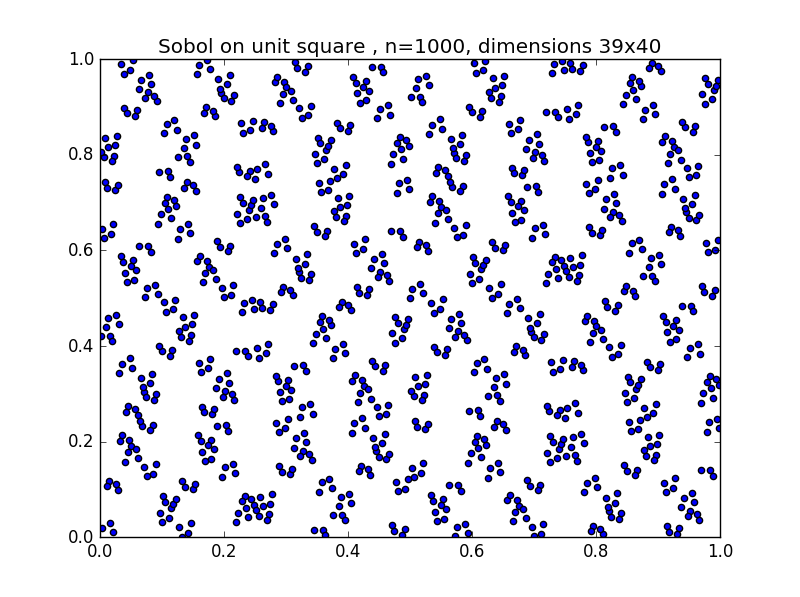
\includegraphics[scale=0.4]{figure_4-sobol 1000 dimensions 39x40.png}
	\caption{Suite de Sobol sous plusieurs dimensions}	
\end{figure}
\clearpage

Comme on peut voir sur la graphes précédents, la suite de Sobol présente beaucoup moins de dégradation en hautes dimensions comparés avec la suite de Halton.\\

Nous comparerons un peu plus loin dans ce document les avantages et inconvénients de chaque suite pour pouvoir en utiliser une suivant la situation du problème à résoudre.

\end{document}